\documentclass[draftclsnofoot, onecolumn, compsoc, 10pt]{IEEEtran}

\title{\huge Software Requirements Specifications}
\author{Oregon State University\\CS 461\\2017-2018\\\\Prepared By:\\ Kyle Prouty\\Hayden Anderson\\}
\usepackage{lscape}
\usepackage{rotating}
\usepackage{titling}
\usepackage[margin=0.75in]{geometry}
\usepackage{graphicx}
\usepackage{placeins}
\usepackage{url}
\usepackage{setspace}
\geometry{textheight=9.5in, textwidth=7in}
\graphicspath{ {images/} }
\linespread{1.0}
\parindent=0.0in
\parskip=0.2in


% 1. Fill in these details
\def \CapstoneTeamName{		Rodents Of Unusual Size}
\def \CapstoneTeamNumber{		46}
\def \GroupMemberOne{			Hayden Anderson}
\def \GroupMemberTwo{			Kyle Prouty}
\def \CapstoneProjectName{		Project ROUS}
\def \CapstoneSponsorCompany{	HP, Inc}
\def \CapstoneSponsorPerson{	Lonnie Mandigo}

% 2. Uncomment the appropriate line below so that the document type works
\def \DocType{  %Problem Statement
				Requirements Document
				%Technology Review
				%Design Document
				%Progress Report
				}
			
\newcommand{\NameSigPair}[1]{\par
\makebox[2.75in][r]{#1} \hfil 	\makebox[3.25in]{\makebox[2.25in]{\hrulefill} \hfill		\makebox[.75in]{\hrulefill}}
\par\vspace{-12pt} \textit{\tiny\noindent
\makebox[2.75in]{} \hfil		\makebox[3.25in]{\makebox[2.25in][r]{Signature} \hfill	\makebox[.75in][r]{Date}}}}
% 3. If the document is not to be signed, uncomment the RENEWcommand below
%\renewcommand{\NameSigPair}[1]{#1}

% For future reference, at least, here are a few more thoughts on requirements vs. design decisions…
 
% In a requirements document, any assertion made must be traceable to a stakeholder.
% A stakeholder is anyone (actually any role) who will have to live with the system once it’s implemented.
% The implementation team is not a stakeholder unless it has a long term commitment to the result (we can talk about what this looks like when it happens).
% Constraints imposed by the environment (for example standards, laws, etc.) represent a special kind stakeholder.
% Future developers are an interesting kind of stakeholder if you’re doing “platform” work. This is a pretty different kind of commitment though.
 
% Here are some useful tests whenever you put an assertion into a requirements document…
% Does this assertion specify a particular technology (Unix, Docker, etc.)?  If so, which stakeholder said that it was required?  If not, then it’s likely a design decision.
% Does this assertion specify a particular architectural pattern (e.g. distributed autonomous nodes)?  If so, which stakeholder said it was required and did they explain why?  If not, then it’s likely a design decision.
% Does this assertion specify a particular implementation approach or process?  …
 
% This, of course, only helps with what should or shouldn’t be in an SRS.
 
% What’s useful to have in an SRS includes the following…
% A high-level narrative (1 to 2 paragraphs) that you would use to introduce the system to someone unfamiliar with it after it has been implemented.
% A description of the context of the system.  (I.e. things not part of the system that interact with the system).  This will include a list of the stakeholders but will likely also include other external entities (which will provide constraints).
% A description of each stakeholder; who they are, what circumstance they are in when interacting with the system, why they care.
% A description of each external non-stakeholder entity; what it does and why it’s there.
% For each stakeholder, what are the outcomes that they expect from the system given a particular circumstance? (These are the requirements.)
% For each external entity, what are the constraints that they impose on the system?
% Note that requirements aren’t always “functional” (what the system did). Sometimes they’re “non-functional” (how the system did it).
% Anything required to effectively read the document such as definitions, a table-of-contents, etc.
 
% To test the quality of your requirements, I recommend asking yourself at least the following two questions …
% How can I measure it?  -  Sometimes that’s as simple as exists/doesn’t exist.
% How can I test it? – Sometimes that’s as simple as the product owner saying “Good enough”


% Lonnies description statement about project:
% Loosely coupled cyber physical systems (aka, the Internet of Things) open the door to huge opportunities and huge challenges for computing and communications as these system grow in complexity and capability. It isn't reasonable for these devices to "call home" (e.g. call a cloud service) for every coordination decision and it isn't reasonable for collections of these devices to have rigid logical configurations. What is needed is a technology that enables collections of smart enough devices to self-organize and collaboratively execute in support of achieving an objective. Capstone students will design or identify and acquire a collection "smart enough" devices and develop a proof-of-concept where these devices create an ad hoc organization and collaborate on an objective. A version we've done in the past is to coordinate a set of smart light bulbs in order to achieve a particular light level based on an occupant's preferences or current task. A different use case than this needs to be created.


%%%%%%%%%%%%%%%%%%%%%%%%%%%%%%%%%%%%%%%
\begin{document}
\begin{titlepage}
    \pagenumbering{gobble}
    \begin{singlespace}
%     	\includegraphics[height=4cm]{coe_v_spot1}
        \hfill 
        % 4. If you have a logo, use this includegraphics command to put it on the coversheet.
        %\includegraphics[height=4cm]{CompanyLogo}   
        \par\vspace{.2in}
        \centering
        \scshape{
            \huge CS Capstone \DocType \par
            {\large\today}\par
            \vspace{.5in}
            \textbf{\Huge\CapstoneProjectName}\par
            \vfill
            {\large Prepared for}\par
            \Huge \CapstoneSponsorCompany\par
            \vspace{5pt}
            {\Large\NameSigPair{\CapstoneSponsorPerson}\par}
            {\large Prepared by }\par
            Group\CapstoneTeamNumber\par
            % 5. comment out the line below this one if you do not wish to name your team
            \CapstoneTeamName\par 
            \vspace{5pt}
            {\Large
                \NameSigPair{\GroupMemberOne}\par
                \NameSigPair{\GroupMemberTwo}\par
            }
            \vspace{20pt}
        }
        \begin{abstract}
\noindent This document will give an overview of software dependencies, the intended function, characteristics, constraints, and assumptions of the framework. The first section is geared more towards giving a high level examination of the framework. The third and fourth sections, Specific Requirements and Software System Attributes, are intended for a more technical audience who would be familiar with the technical aspects and relevant terminology of this framework.  
        \end{abstract}     
    \end{singlespace}
\end{titlepage}
\newpage
\pagenumbering{arabic}
\clearpage 
\tableofcontents
\pagebreak



\section{Introduction}
\subsection{Purpose} 
The purpose of this document is to layout and define the objective and details of the framework to be developed. This document will specify an overall description, specific requirements, and software system attributes of this framework. This document details what the project's end product will do for an end user. The intended audience for this document includes any relevant stakeholders. 

\subsection{Scope}
The goal of this framework will be to allow a user to input an objective into the framework, see how the framework organizes on that objective, and then view the result of that organization. This framework will be able to self organize when encountering a node that is mistrusted. Overall, this framework will enforce a robust system that can mitigate nodes that are untrusted by the framework.

% Nodes will carryout an objective based on the services available. Three main goals will be achieved in order to complete the main objective. First, the framework will enable nodes to communicate with each other and will have the ability to share processes. Next, an objective will be able to be input into the framework. Finally, the nodes will self organize on the objective and output the results to the user.
% The services needed to finish the job will propagate through the system to find the nodes that can carryout each service. Once each service in an objective has a node that can carry them out. The node that received the user input will output where the piece(s) of the objective are being completed. The framework will be able to (re)direct services and jobs away from established security threatened nodes.  
% \centering{
% 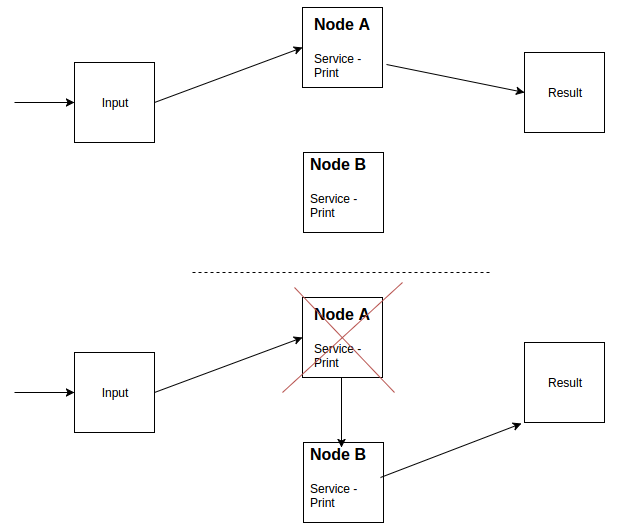
\includegraphics[scale=0.4]{img_1}
% }

\subsection{Definitions, Acronyms, Abbreviations}
\bgroup
\def\arraystretch{1.5}
\resizebox{\textwidth}{!}{
\begin{tabular}{| p{10.0cm} | p{10.0cm} |}
\hline
\bf{Term} & \bf{Definition}\\ 
\hline
Stakeholder  & User of the Project ROUS \\
\hline
Project ROUS  & framework that includes all aspects of input, output, software, hardware, and user interface \\
\hline
User  & The person who would use this at its completion that doesn’t know how it works   \\
\hline
Node  & Our built device that acts as a layer between IoT enabled machines and other nodes \\ 
\hline
%Docker &  A container of isolated code \\
%\hline
%Unix & An open-source operating system \\
%\hline
Rodents of Unusual Size (ROUS)  &  Project name  \\ 
\hline
Graphical User Interface (GUI)  & A visual representation for the user to interact with  \\ 
\hline
Internet of Things (IoT)  & A blanket statement to describe objects that have been made to be able to connect to the Internet.  \\ 
\hline
%Model View Controller (MVC)  &  A software architecture for implementing an interface for the user  \\ 
%\hline
Local Area Network (LAN) & A network of connected devices contained within a small geographical space  \\
\hline
%Message Queue Telemetry Transport (MQTT) & lightweight TCP/IP protocol\\
%\hline
%Advanced RISC Machine (ARM) architecture & computer processor architecture \\
%\hline
\end{tabular}
}
\egroup

\subsection{References}
IEEE. IEEE Std 830-1998 IEEE Recommended Practice for Software Requirements Specifications. IEEE Computer Society,1998.

\subsection{Overview}
The next section of this document, Overall Description, gives a high level view of the framework. The third and fourth sections, Specific Requirements and Software System Attributes, will give a slightly more in-depth examination of the different aspects of the framework. 

% In the next section of this document, Overall Description, will give an overview of software dependencies, the intended function, characteristics, constraints, and assumptions of the framework. This section is geared more towards giving a more high level examination of the framework. The third and fourth sections, Specific Requirements and Software System Attributes, is intended for more of a technical audience who would be familiar with the technical aspects and relevant terminology of this framework. 

\section{Overall Description}
\subsection{Product Perspective}
The framework will be a middle layer between the user and the result. Users will input a structured objective into the framework, the framework will self organize on that objective, and then the user will see the result. For this framework a structured objective will be a print job. This frameworks specific use case will be to allow users to input print jobs into the framework, have the framework organize on that print job, and then view the results of that print job.


\begin{figure}[!htb]
\centering
	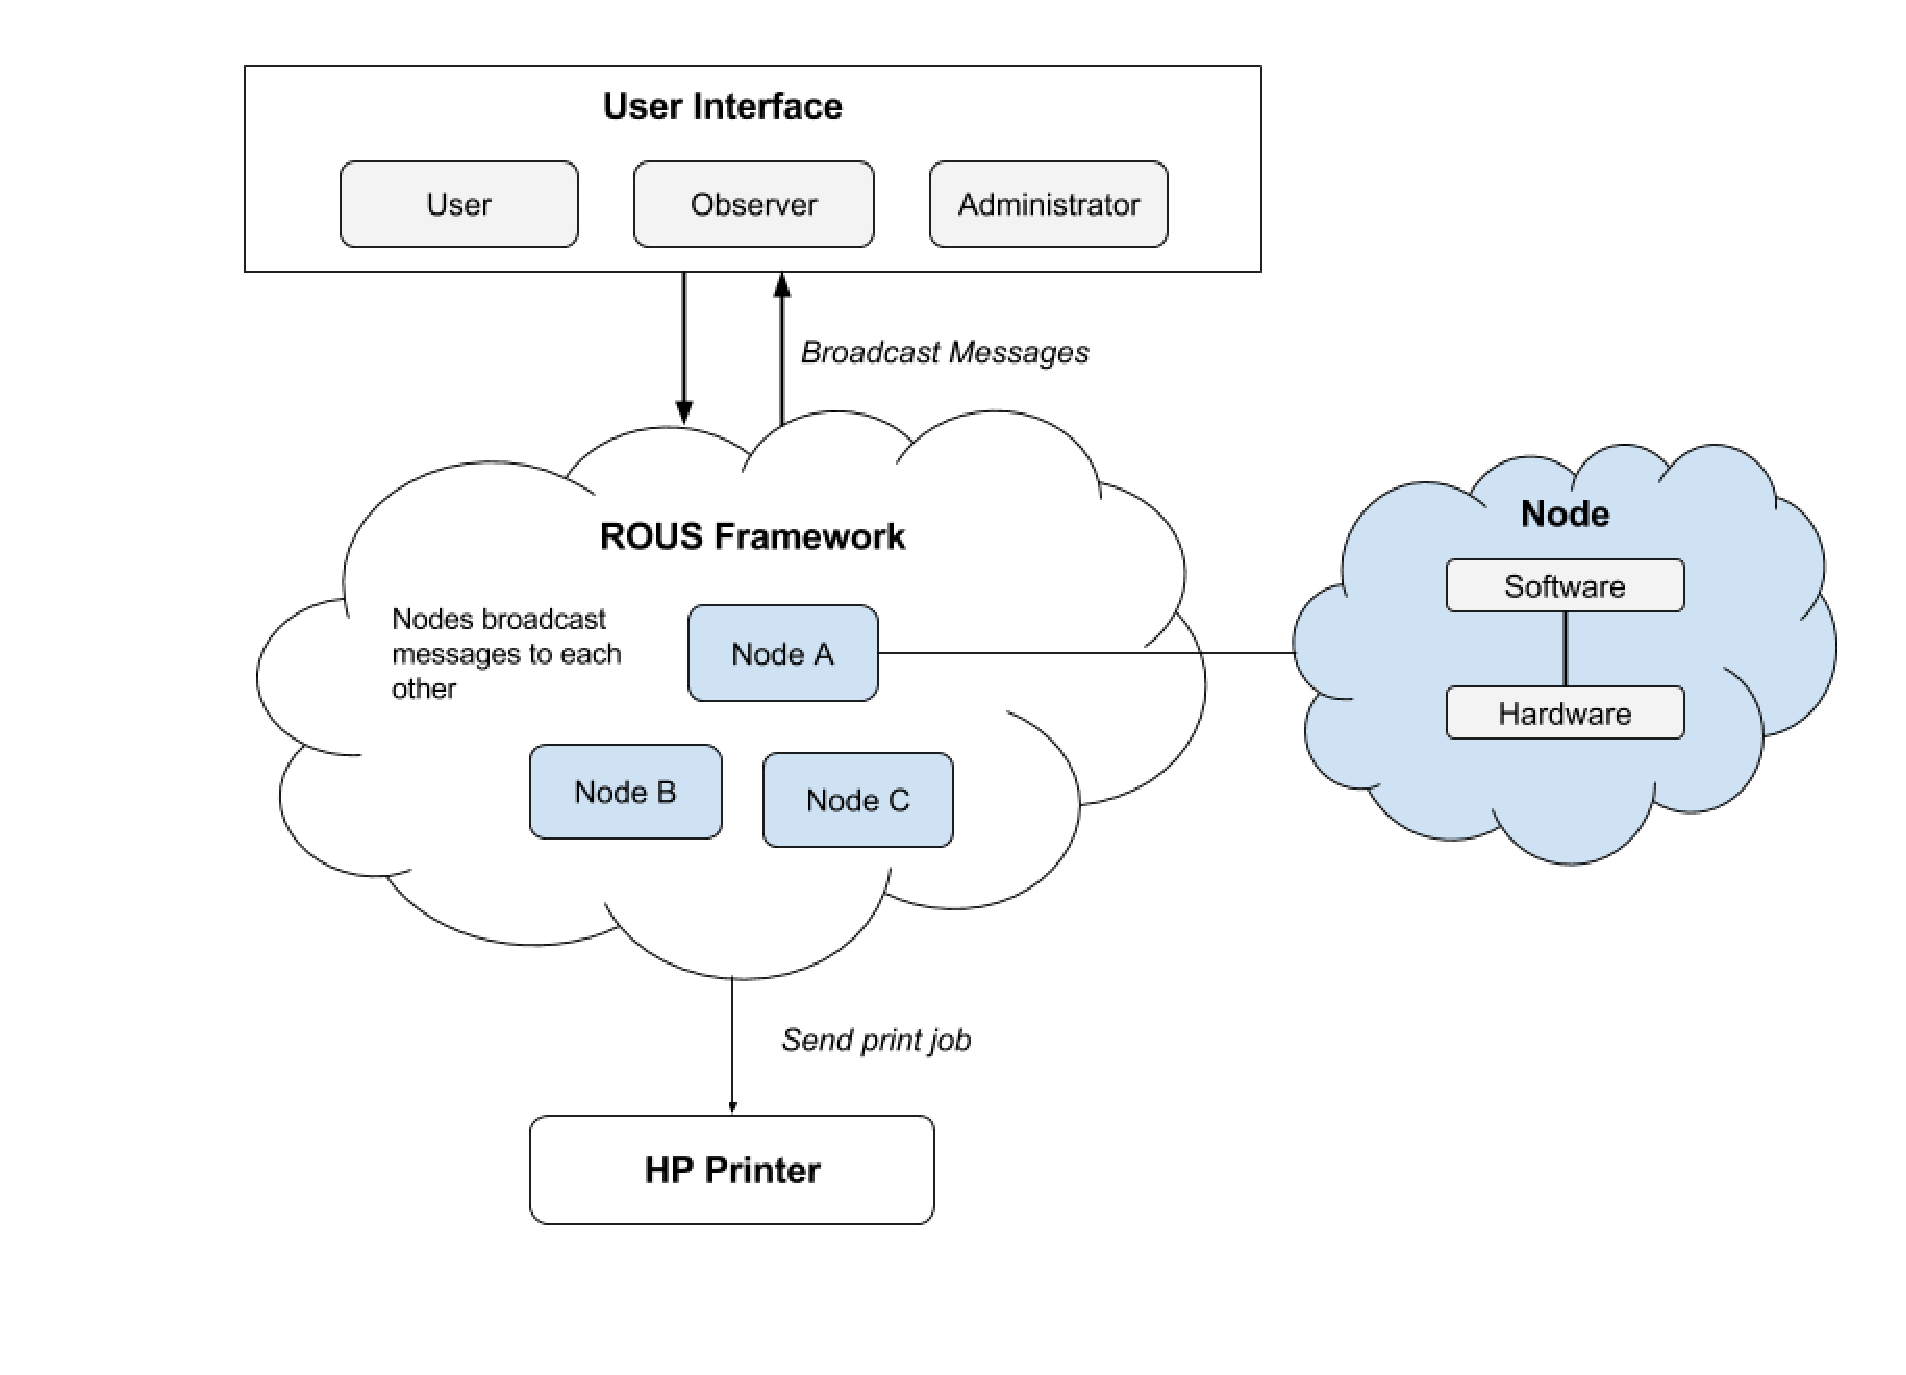
\includegraphics[width=1.0\textwidth]{context}
	\caption{This figure shows a context view of the overall framework. It describes the sources of input and output to the system.}
  
\end{figure}

\subsubsection{System Interfaces}
The primary system interface that users will interact with will be a software based user interface. Users of this system will not interact at the system interface level.

%%%NEED NEW ONE, I have no idea -Hayden

\subsubsection{User Interfaces}
\begin{itemize}
\item A command line based interface to modify framework settings.\\
\item A GUI that will allow users to input objectives and view the results. Outputted results will have clear visualization that is readable and understandable to relevant stakeholders. 
% \item A web based gui that will interface between an administrator and the nodes. This graphical interface is used to show the nodes in the framework, the services each node offers, and the nodes connections with each other.\\ 
% \item A web based gui that will interface between a user and the nodes. This graphical interface is used to let a user upload a file into the collection of nodes and view the status of the result.
\end{itemize}

\subsubsection{Hardware Interfaces}
No hardware specifications required. This framework will be build in software.
% This framework will use a combination of various ARM based micro-controllers. These micro-controllers must have the functionality to communicate with 802.11 b/g/n wireless LAN communication protocols.

\subsubsection{Software Interfaces}
Framework will be built in software. %It will only interact with the Unix based operating system. 
Users will interact with the framework through a software user interface.

%\subsubsection{Communications Interfaces} %%blocked out due to Lonnie's request
%The network protocol that is required by this framework is Ethernet, with communication protocols TCP/IP and 802.11 b/g/n wireless LAN.

%\subsubsection{Memory constraints}
%The framework is only constrained to what the hardware that is used will allow.
 
\subsubsection{Operations}%NEEDS LESS DESIGN (not yelling just need a visual cue so I see this when scrolling)
This section details the operations required by the stakeholders for the system to do what it was designed for.

In order for the system to accomplish its objective the end user will need to:
\begin{itemize}
\item Input a structured objective into the framework 
\item View the results of the objective 
\end{itemize}

In order for the system to accomplish its objective the hacker will need to:
\begin{itemize}
\item Input a source of mistrust into the framework 
\item View the system state 
\item View the configuration settings 
\end{itemize}

In order for the system to accomplish its objective the administrator will need to:
\begin{itemize}
\item Change configuration settings on a specific node 
\item View the system state 
\item View the configuration settings 
\end{itemize}

The system will:
\begin{itemize}
\item Enable nodes to self organize on a structured objective 
% \item Propagate the objective to each node by the services required to be finished by the objective \\
% \item Allow the objective to be completed by other nodes if there is a node with corrupted or infected services \\
\end{itemize}

\subsubsection{Site Adaptation Requirements}
There are no site adaptations required.


\subsection{Product Functions}
%intro blurb
Below is a list of the basic functions that this framework will perform. It is a high level view of the functions that the framework will be able to execute.
\begin{itemize}
\item Send an objective to the framework
\item Display the results of the objective
\item Send a source of mistrust to the framework
\item Display the system state 
\item User interface that visualizes the results of an objective
\item Framework can self-organize on an objective
\end{itemize}
In the figure below you will see a basic high level description of how this framework will function.
\begin{figure}[!htb]
  \centering
    \includegraphics[width=1.0\textwidth]{functions}
  \caption{The right image shows an objective A being input into the framework, and its corresponding result A. In the left image, it shows the same objective A going to the same node 1, but this time node 1 is mistrusted. Now, the nodes have to self organize and reroute the objective to a different node 2 which achieves the same result A. }
\end{figure}
\FloatBarrier

\subsection{User Characteristics} 
%The users of this framework will be our relevant stakeholders. These users will have had some level of formal technical education.

The users of this framework include the job submitter(end user), the hacker, and the administrator, and the observer.

The job submitter will be the end user that needs the utility that our system provides. They will use the system to send their job's objective for the desired outcome. The user will input a task and the system will carryout the objective.

The hacker is an unexpected stakeholder that is inherited from the inherent nature of being part of the Internet of Things. The end product will see the hacker as an outside source that corrupts services provided by the framework. 
% Within the scope of our product the hacker will press a button to simulate a service corruption.

The administrators are expected to have some level of formal technical education. They are able to understand how the system works as a whole and individually.

Observers are the passersby that can watch the system from the user interface. The observer will be able to understand what is connected and what each node is capable of.

\subsection{Constraints}
This framework will not communicate to outside sources for any of its configuration settings. Each individual node must be able to lead the framework on decisions required. Nodes cannot utilize an external database for its inner information structure. Nodes cannot exchange information by using an external database.

%\subsection{Assumptions and Dependencies}
%This document and current requirements assume that each hardware device used has Ethernet capabilities, also large enough memory and storage to fit the frameworks docker image. Physical devices will have the resources available to run the docker image. These physical devices will also be able to handle the frameworks user interface.
%Attempt #2: This document and current requirements assume that each stakeholder that takes place within the project's setting be familiar with setting up a connection to a device with their computer

%attempt #3: This framework assumes that the user knows to send a print job to a device. The network also requires a wireless capable device; specifically a printer for this project. The user's role, in terms of username and ID, are previously determined. Creating a user account that is valid within the system is a stretch goal.


%need a new one that doesn't have to do with docker images. focus for more of the end user's maybe? like assume the user has IoT devices that can communicate with our nodes. and that there is a hacker trying to disrupt services. and that there is an objective from a user that needs to be accomplished.

\subsection{Apportioning of Requirements}
Refer to Gantt chart in figure below for this information.
\begin{landscape}
	\begin{figure}[!htb]
		\caption{Gantt Chart}
		\centering
			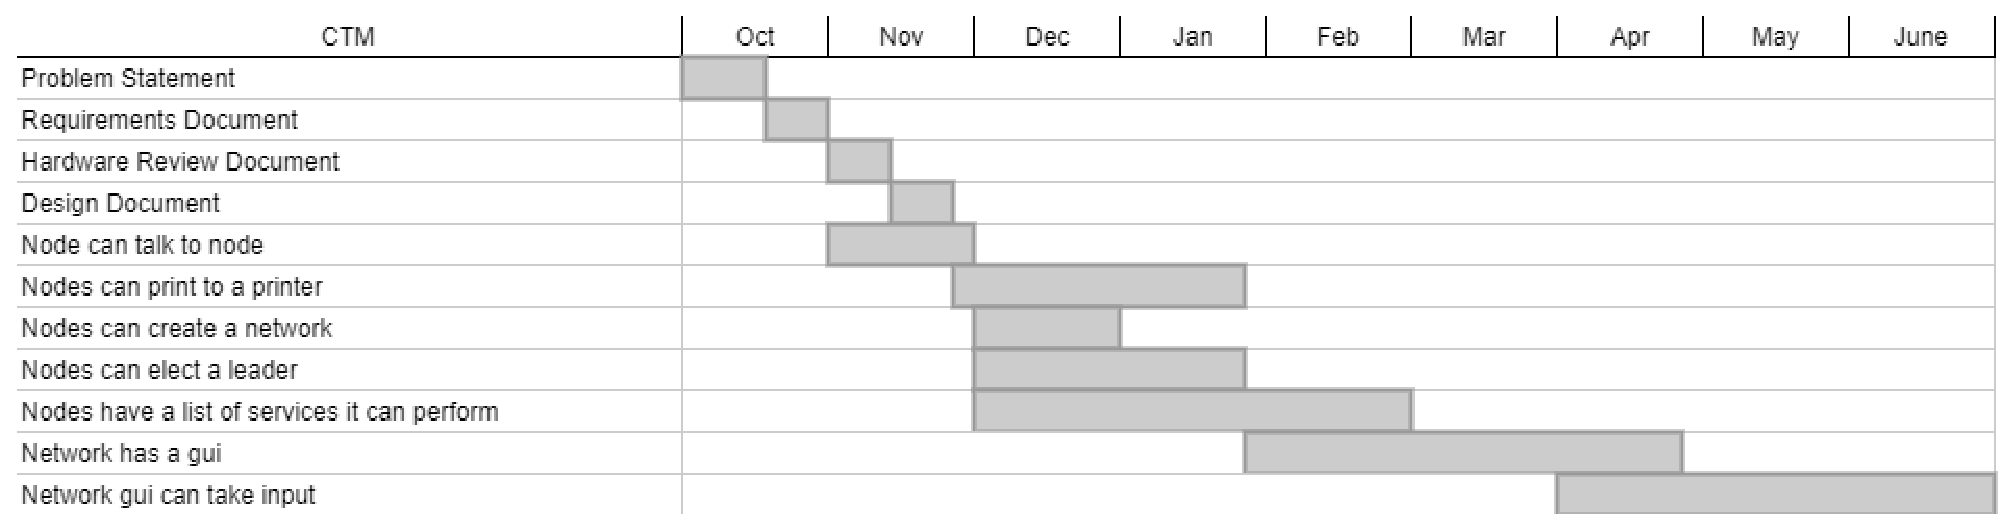
\includegraphics[scale=.7]{chart.eps}
	\end{figure}
\end{landscape}
\FloatBarrier

\section{Specific Requirements}
\subsection{External Interfaces}
\begin{itemize}
\item Input:
	\begin{itemize}
	\item Objective 
    \item Source of Mistrust
	\end{itemize}
\item Output:
	\begin{itemize}
	\item Result of Objective
    \item System state
	\end{itemize}
\end{itemize}

\subsection{Functions}
The system shall ...
\begin{itemize}
\item Enable nodes to self organize on a structured objective
\item Allow an objective to be input
\item Allow a source of mistrust to be input
\item Output readable configuration data
\item Output readable system state data
\item Output readable results of objective
\item Automatically validate and connect to authorized nodes
\item Allow nodes to share objectives with each other
\item Framework state changes based on the input of a source of mistrust
\item Have a user interface
\item Offer a print service
\end{itemize}

\subsection{Performance Requirements}
This framework will support at a minimum two nodes. Each objective received by the framework from the user will start and execute on 90\% of the services required by the objective given. Only one user will be able to input an objective at a time. Objectives can be queued and executed consecutively. Each node will support, at a minimum, a print service. A user will have to wait for an objective to complete before inputing a new objective. 

\subsection{Logical Database Requirements}
There are no database requirements. 

\subsection{Design Constraints}
There is not an external database to which the framework should be writing to or retrieving from to carry out objectives. The network must be able to send a parallel job to two monochrome printers. The network must be able to send a singular job to a color printer with parallel being a stretch goal. Logging of framework events to an external database.

\subsection{Standards Compliance}
This framework will need to stay compliant with general industry standards.
%%%or should we just have it not need to be compliant but actually use it, since it staying compliant is a design choice? 

%Kyle:	I like it how you have it


\section{Software System Attributes}
\subsection{Reliability}
The reliability of this framework will be measured by the user's ability to:
\begin{itemize}
\item input an objective into the framework
\item see the objective being organized in the framework
\item view the results of that organization
\end{itemize} 
This allows the user to visually watch the (lifespan) of their objective and its effects on the system.


\subsection{Security}
%The framework will only accept authorized nodes. Nodes will be password protected and will only accept objectives and sources of mistrust from verified users.

The framework will only accept authorized nodes. Nodes will only accept objectives and sources of mistrust from verified users.

\subsection{Maintainability}
%Code will be well commented and readable to 8 out of 10 software developers. A MVC design scheme will be implemented. File structure will be well organized and self explanatory to navigate.

Code will be well commented and readable for someone that has college graduate programming skills. The file structure will be well organized and self explanatory to navigate. 

\subsection{Portability}
This framework will be fully portable to any system that can run a Docker container (stretch goal). 

\subsection{Other Requirements}
No additional requirements for this framework.

\end{document}